% FiCRNN, figure 2: simplified view of the recurrence over T windows
\documentclass[border=8pt]{standalone}
\usepackage{amsmath,amssymb}
\usepackage{tikz}
\usetikzlibrary{positioning,arrows.meta,fit,backgrounds,calc,decorations.pathreplacing}

\definecolor{cIn}{HTML}{E8EEF7}     \definecolor{cInD}{HTML}{3B5B8C}
\definecolor{cCnn}{HTML}{E6F2EA}    \definecolor{cCnnD}{HTML}{2E7D4F}
\definecolor{cFilm}{HTML}{FCEBDD}   \definecolor{cFilmD}{HTML}{C0622B}
\definecolor{cRnn}{HTML}{EFE7F6}    \definecolor{cRnnD}{HTML}{6A4C93}

\begin{document}
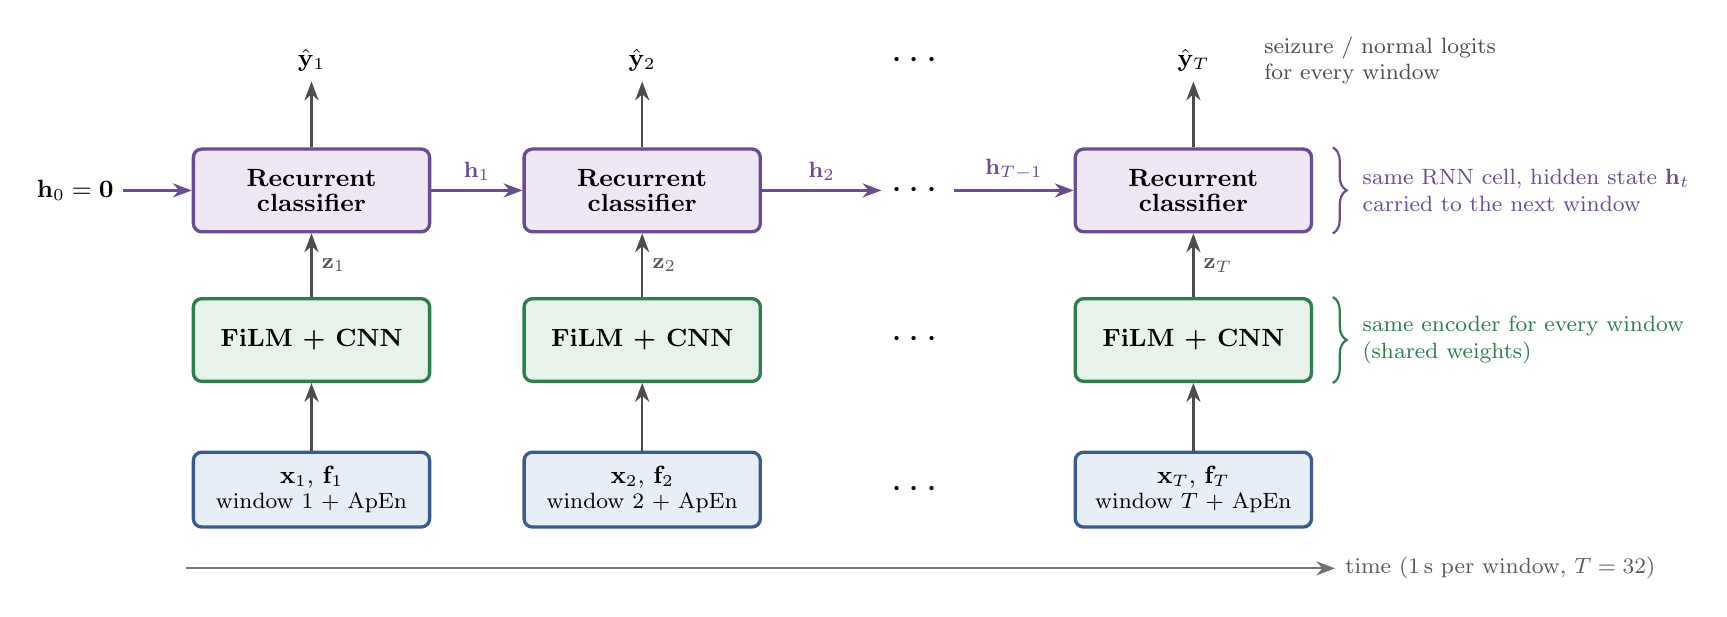
\begin{tikzpicture}[
  font=\small,
  >={Stealth[length=2.4mm]},
  arr/.style={->, thick, draw=black!70},
  box/.style={draw, rounded corners=3pt, very thick, align=center, inner sep=4pt,
              minimum width=3.0cm},
  inp/.style={box, draw=cInD, fill=cIn, minimum height=0.95cm},
  enc/.style={box, draw=cCnnD, fill=cCnn, minimum height=1.05cm},
  rec/.style={box, draw=cRnnD, fill=cRnn, minimum height=1.05cm},
  lab/.style={font=\footnotesize, text=black!65},
]

\foreach \t/\x/\lab in {1/0/1, 2/4.2/2, T/11.2/T}{
  \node[inp] (in\t) at (\x, 0)   {$\mathbf{x}_{\lab}$, $\mathbf{f}_{\lab}$\\[-2pt]{\footnotesize window $\lab$ + ApEn}};
  \node[enc] (e\t)  at (\x, 1.9) {\textbf{FiLM + CNN}};
  \node[rec] (r\t)  at (\x, 3.8) {\textbf{Recurrent}\\[-2pt]\textbf{classifier}};
  \node      (y\t)  at (\x, 5.45) {$\hat{\mathbf{y}}_{\lab}$};
  \draw[arr] (in\t) -- (e\t);
  \draw[arr] (e\t) -- node[right, lab] {$\mathbf{z}_{\lab}$} (r\t);
  \draw[arr] (r\t) -- (y\t);
}

% recurrence
\node (h0) at (-3.0, 3.8) {$\mathbf{h}_0=\mathbf{0}$};
\draw[arr, draw=cRnnD] (h0) -- (r1);
\draw[arr, draw=cRnnD] (r1) -- node[above, lab, text=cRnnD] {$\mathbf{h}_1$} (r2);
\node (rd) at (7.7, 3.8) {\Large$\cdots$};
\draw[arr, draw=cRnnD] (r2) -- node[above, lab, text=cRnnD] {$\mathbf{h}_2$} (rd);
\draw[arr, draw=cRnnD] (rd) -- node[above, lab, text=cRnnD] {$\mathbf{h}_{T-1}$} (rT);
\node at (7.7, 1.9) {\Large$\cdots$};
\node at (7.7, 0)   {\Large$\cdots$};
\node at (7.7, 5.45){\Large$\cdots$};

% row labels on the right
\draw[decorate, decoration={brace, amplitude=5pt}, thick, cCnnD]
  ($(eT.north east)+(0.25,0)$) -- ($(eT.south east)+(0.25,0)$)
  node[midway, right=7pt, align=left, font=\footnotesize, text=cCnnD]
  {same encoder for every window\\(shared weights)};
\draw[decorate, decoration={brace, amplitude=5pt}, thick, cRnnD]
  ($(rT.north east)+(0.25,0)$) -- ($(rT.south east)+(0.25,0)$)
  node[midway, right=7pt, align=left, font=\footnotesize, text=cRnnD]
  {same RNN cell, hidden state $\mathbf{h}_t$\\carried to the next window};
\node[right=0.45cm of yT, align=left, font=\footnotesize, text=black!70]
  {seizure / normal logits\\for every window};

% time axis
\draw[->, thick, black!55] (-1.6, -1.0) -- (13.0, -1.0)
  node[right, font=\footnotesize, text=black!65] {time (1\,s per window, $T=32$)};

\end{tikzpicture}
\end{document}
